\documentclass[a4paper]{article}

\usepackage[english]{babel}
\usepackage[utf8]{inputenc}
\usepackage{amsmath}
\usepackage{graphicx}
\usepackage[colorinlistoftodos]{todonotes}
\usepackage{listings}
\usepackage{hyperref}
\usepackage{changepage}

\title{Statistical Inference Course Project, part 2: Hypothesis Testing}

\author{Daniel Kudlowiez Franch}

\begin{document}
\maketitle

In this part of the project, the Tooth Growth data contained in R's datasets library will be analyzed. This data is composed by 60 observations of tooth length in 10 guinea pigs at three dose levels of Vitamin C (0.5, 1 and 2 mg) with two delivery methods (ascorbic acid or orange juice).

\section*{Exploratory Data Analysis}

The following code makes an initial exploratory analysis of the data:

\begin{small}
\begin{lstlisting}[frame = single]
library(ggplot2)
library(datasets)

tg <- ToothGrowth
ggplot(data = tg,
       aes(x = as.factor(dose),
           y = len,
           fill = supp)) +
    geom_bar(stat = "identity",) +
    facet_grid(.~supp) +
    xlab("Dose in Miligrams") +
    ylab("Tooth Length") +
    guides(fill = guide_legend(title = "Supplement Type"))
\end{lstlisting}
\end{small}

\begin{figure}[h!]
\centering
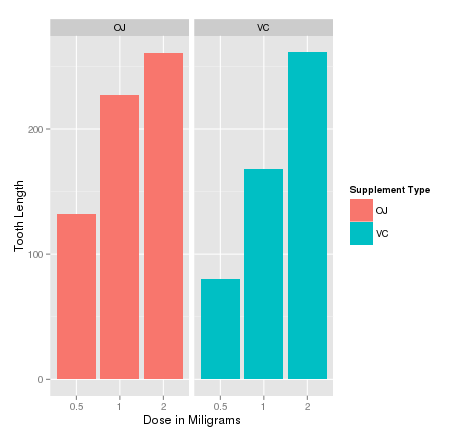
\includegraphics[width = 0.46\textwidth]{part2.png}
\end{figure}

It is possible to note certain correlation between tooth length and Vitamin C dose level, independent of delivery method.

\section*{Hypothesis Testing}

The standard error estimate will generally not be too accurate as the subsets are smaller than 30 observations. For this reason, the hypothesis testing will be done with the t-test.

The first test is done to verify if the difference between tooth length of guinea pigs who received Vitamin C through different delivery methods is statistically zero. This is done with a t-test with unequal variance of the two samples:

\begin{small}
\begin{flushleft}
\begin{tabular}{|c|c|c|c|c|c|c|c|}
\hline
estimate & estimate1 & estimate2 & statistic & p.value & parameter & conf.low & conf.high \\ \hline
3.7 & 20.66333 & 16.96333 & 1.915268 & 0.06063451 & 55.30943 & -0.1710156 &  7.571016 \\
\hline
\end{tabular}
\end{flushleft}
\end{small}

The p-value found is approximately 0.061, which is higher than the significance of 0.05, thus we fail to reject the null-hypothesis. Therefore, it is not possible to say that the average difference in tooth length of guinea pigs that received the different supplements is different from zero.

The next step is to compare all factor levels combinations using 3 t-tests. The null hypothesis for each test will be that the difference between tooth length for each factor is 0.

The following table summarizes each of the tests that was performed:

\begin{small}
\begin{adjustwidth}{-1.5cm}{0.5cm}
\begin{flushleft}
\begin{tabular}{|c|c|c|c|c|c|c|c|c|}
\hline
null hypothesis & estimate & estimate1 & estimate2 & statistic & p.value & parameter & conf.low & conf.high \\ \hline
2mg - 1mg = 0 & 6.365 & 26.100 & 19.735 & 4.900484 & 1.906430e-05 & 37.10109 & 3.733519 & 8.996481 \\ \hline
2mg - 0.5mg = 0 & 15.495 & 26.100 & 10.605 & 11.799046 & 4.397525e-14 & 36.88259 & 12.833833 & 18.156167 \\ \hline
1mg - 0.5mg = 0 & 9.130 & 19.735 & 10.605 & 6.476648 & 1.268301e-07 & 37.98641 & 6.276219 & 11.983781 \\
\hline
\end{tabular}
\end{flushleft}
\end{adjustwidth}
\end{small}

It is possible to see from the table that all three p-values are smaller than the significance level adopted, which means that we reject the null hypothesis in all cases. Therefore, the data shows strong evidence that the average tooth length of the subject guinea pigs is different for each Vitamin C dose level. 

A possible interpretation of the first test in the table is that we have 95\% of confidence that the difference between average tooth length of guinea pigs that received a 2mg dose of Vitamin C is on average 3.733 to 9mm higher than those who received a 1mg dose.

\section*{Conclusion}

From the tooth growth data we could analyze and conclude that the observed difference of average tooth length across different types of supplement is statistically not different from 0.

On the other hand, the same observations across different dose levels is significantly different from zero.

Further studies could include pairwise t-tests of different combinations of supplements and dose levels.

\newpage

\section*{Appendix}

Here is the source code used to obtain both the exploratory data analysis' graphs and the t-tests results:

\begin{small}
\begin{lstlisting}[frame = single]
library(ggplot2)
library(datasets)
library(broom)
library(dplyr)

#Loading the Tooth Growth data:
tg <- ToothGrowth

#Exploratory Analysis:
ggplot(data = tg,
       aes(x = as.factor(dose),
           y = len,
           fill = supp)) +
    geom_bar(stat = "identity") +
    facet_grid(.~supp) +
    xlab("Dose in Miligrams") +
    ylab("Tooth Length") +
    guides(fill = guide_legend(title = "Supplement Type"))

#T-Test for difference in tooth length across supplement types:
t_supp <- t.test(len ~ supp, tg, var.equal = FALSE)
tidy(t_supp)

#Pairwise t-tests for differences in tooth lengths means 
#across dose levels:
pWise <- t.test(tg$len[tg$dose == 2], tg$len[tg$dose == 1]) 
%>% tidy %>%
mutate(null_hypothesis = '2mg - 1mg = 0') %>%
select(9, 1:8)

pWise <- t.test(tg$len[tg$dose == 2], tg$len[tg$dose == 0.5]) 
%>% tidy %>%
mutate(null_hypothesis = '2mg - 0.5mg = 0') %>%
select(9, 1:8) %>%
bind_rows(pWise, .)

pWise <- t.test(tg$len[tg$dose == 1], tg$len[tg$dose == 0.5]) 
%>% tidy %>%
mutate(null_hypothesis = '1mg - 0.5mg = 0') %>%
select(9, 1:8) %>%
bind_rows(pWise, .)

print.data.frame(pWise)
\end{lstlisting}
\end{small}

\end{document}